\subsection{The project instance, up to a million pulls}

In the first follow-up (in French, in the \texttt{extensions} folder of the repository) we already ran the four algorithms together with ETC(10) and $\varepsilon_n$-greedy up to $n = 10^5$. The short version: ETC(10) and $\varepsilon_n$-greedy have a tiny median regret but 5 runs out of 200 stay stuck on arm 2 for a long time, so their mean regret is around 2\,000; the index policies never get stuck. Here we only follow KL-UCB and Thompson sampling, but much further, to $n = 10^6$ with 100 runs, to see what really happens to $R_n / \log n$.

\begin{figure}[htbp]
\centering
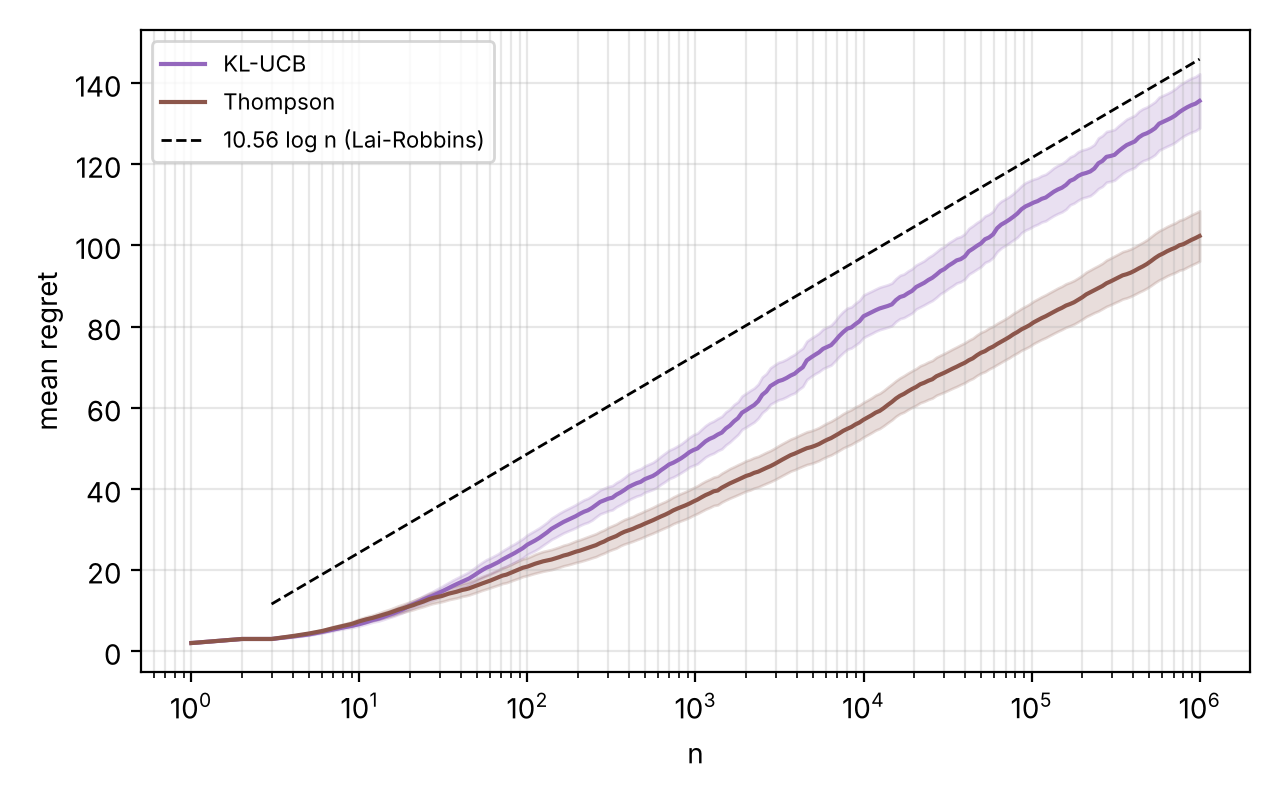
\includegraphics[width=0.66\textwidth]{bandits_long.png}
\caption{Mean regret of KL-UCB and Thompson sampling on the instance $(2, 3, 4)$, 100 runs, with $\pm 2$ standard errors. The dashed line is $C \log n$.}
\label{fig:long}
\end{figure}

At $n = 10^6$ the mean regret is $135.6 \pm 3.3$ for KL-UCB and $102.3 \pm 3.1$ for Thompson sampling (standard errors over runs). Divided by $\log n$ this gives $9.82$ and $7.41$, both \emph{below} $C = 10.56$, which at first looks strange for algorithms that are supposed to be optimal and not better than optimal.

The ratio is the wrong thing to look at, though. If $R_n \approx a \log n + b$, then $R_n / \log n = a + b/\log n$, and $b$ can be negative. A least squares fit of $R_n = a\log n + b$ between $10^4$ and $10^6$ gives $a = 11.9$, $b = -28$ for KL-UCB and $a = 9.8$, $b = -32$ for Thompson sampling. So both curves have a large negative offset, and the slope is what should go to $C$. The slope measured decade by decade tells the rest of the story:

\begin{table}[htbp]
\centering\small
\begin{tabular}{lcccc}
\toprule
decade of $n$ & $10^2$--$10^3$ & $10^3$--$10^4$ & $10^4$--$10^5$ & $10^5$--$10^6$ \\
\midrule
KL-UCB & 9.95 & 14.32 & 12.41 & 11.35 \\
Thompson sampling & 7.13 & 8.39 & 10.03 & 9.45 \\
\bottomrule
\end{tabular}
\caption{Local slope of the mean regret against $\log n$ on each decade (Lai--Robbins constant $C = 10.56$).}
\label{tab:decades}
\end{table}

KL-UCB comes down towards $C$ from above, Thompson sampling goes up towards it from below, and on the last decade both are within about $10\%$ of $10.56$. With 100 runs these local slopes are not very precise (the standard error of the final regret is around 3), so we would not read the second decimal. But the picture is consistent with the theory, and it also says that even a million pulls on a three-armed problem is not really ``asymptotic'' yet. If we had stopped at $n = 10^4$, KL-UCB would have looked $35\%$ worse than the bound in slope and Thompson sampling $20\%$ better.

\subsection{When the variance is wrong}

On the instance $(2, 3, 4)$ of the French follow-up, UCB with $\sigma = 1$ had one of the best \emph{median} regrets (32, only ETC(10) was a bit lower with 30), well below $C \log n$, but with one run out of 200 that stayed on the wrong arm for a long time. We wanted to know if this was luck or something structural. The bound says it cannot be free, so we looked for the instance where it pays.

We use two arms $(\mu - 1, \mu)$ with $\mu \in \{2, 4, 16, 64\}$. The gap is always 1, but the variance grows like $\mu$ and the constant grows with it: $C = 3.26$, $7.30$, $31.3$ and $127.3$. For large $\mu$ the Poisson law is close to a Gaussian with variance $\mu$ and $C \approx 2\mu$, which is also the constant $2\sigma^2/\Delta$ of UCB with the oracle $\sigma = \sqrt{\mu}$. So on this family the oracle UCB should become almost optimal, and UCB with $\sigma = 1$ should become more and more over-confident. 100 runs of $n = 10^5$ pulls for each case.

\begin{table}[htbp]
\centering\small
\setlength{\tabcolsep}{4pt}
\begin{tabular}{lcccccccc}
\toprule
& \multicolumn{2}{c}{$\mu = 2$} & \multicolumn{2}{c}{$\mu = 4$} & \multicolumn{2}{c}{$\mu = 16$} & \multicolumn{2}{c}{$\mu = 64$} \\
\cmidrule(lr){2-3}\cmidrule(lr){4-5}\cmidrule(lr){6-7}\cmidrule(lr){8-9}
& mean & median & mean & median & mean & median & mean & median \\
\midrule
$C \log n$ & \multicolumn{2}{c}{37.5} & \multicolumn{2}{c}{84.1} & \multicolumn{2}{c}{360.7} & \multicolumn{2}{c}{1\,466} \\
UCB ($\sigma = 1$) & 25.2 & 24.5 & 585 & 21.0 & 19\,495 & 19.5 & 38\,066 & 23.5 \\
\quad runs stuck & \multicolumn{2}{c}{0\%} & \multicolumn{2}{c}{1\%} & \multicolumn{2}{c}{20\%} & \multicolumn{2}{c}{38\%} \\
UCB (oracle $\sigma$) & 43.7 & 42.0 & 87.8 & 84.0 & 321 & 300.5 & 1\,124 & 1\,074 \\
KL-UCB & 35.5 & 34.0 & 77.7 & 81.0 & 326 & 318.5 & 1\,122 & 1\,016.5 \\
Thompson & 26.3 & 27.0 & 55.2 & 50.5 & 182 & 160.0 & 657 & 654.5 \\
\bottomrule
\end{tabular}
\caption{Regret at $n = 10^5$ on the two-armed family $(\mu - 1, \mu)$, 100 runs. ``Stuck'' means a final regret above $n/10$. The index policies other than UCB ($\sigma = 1$) never got stuck.}
\label{tab:scale}
\end{table}

\begin{figure}[htbp]
\centering
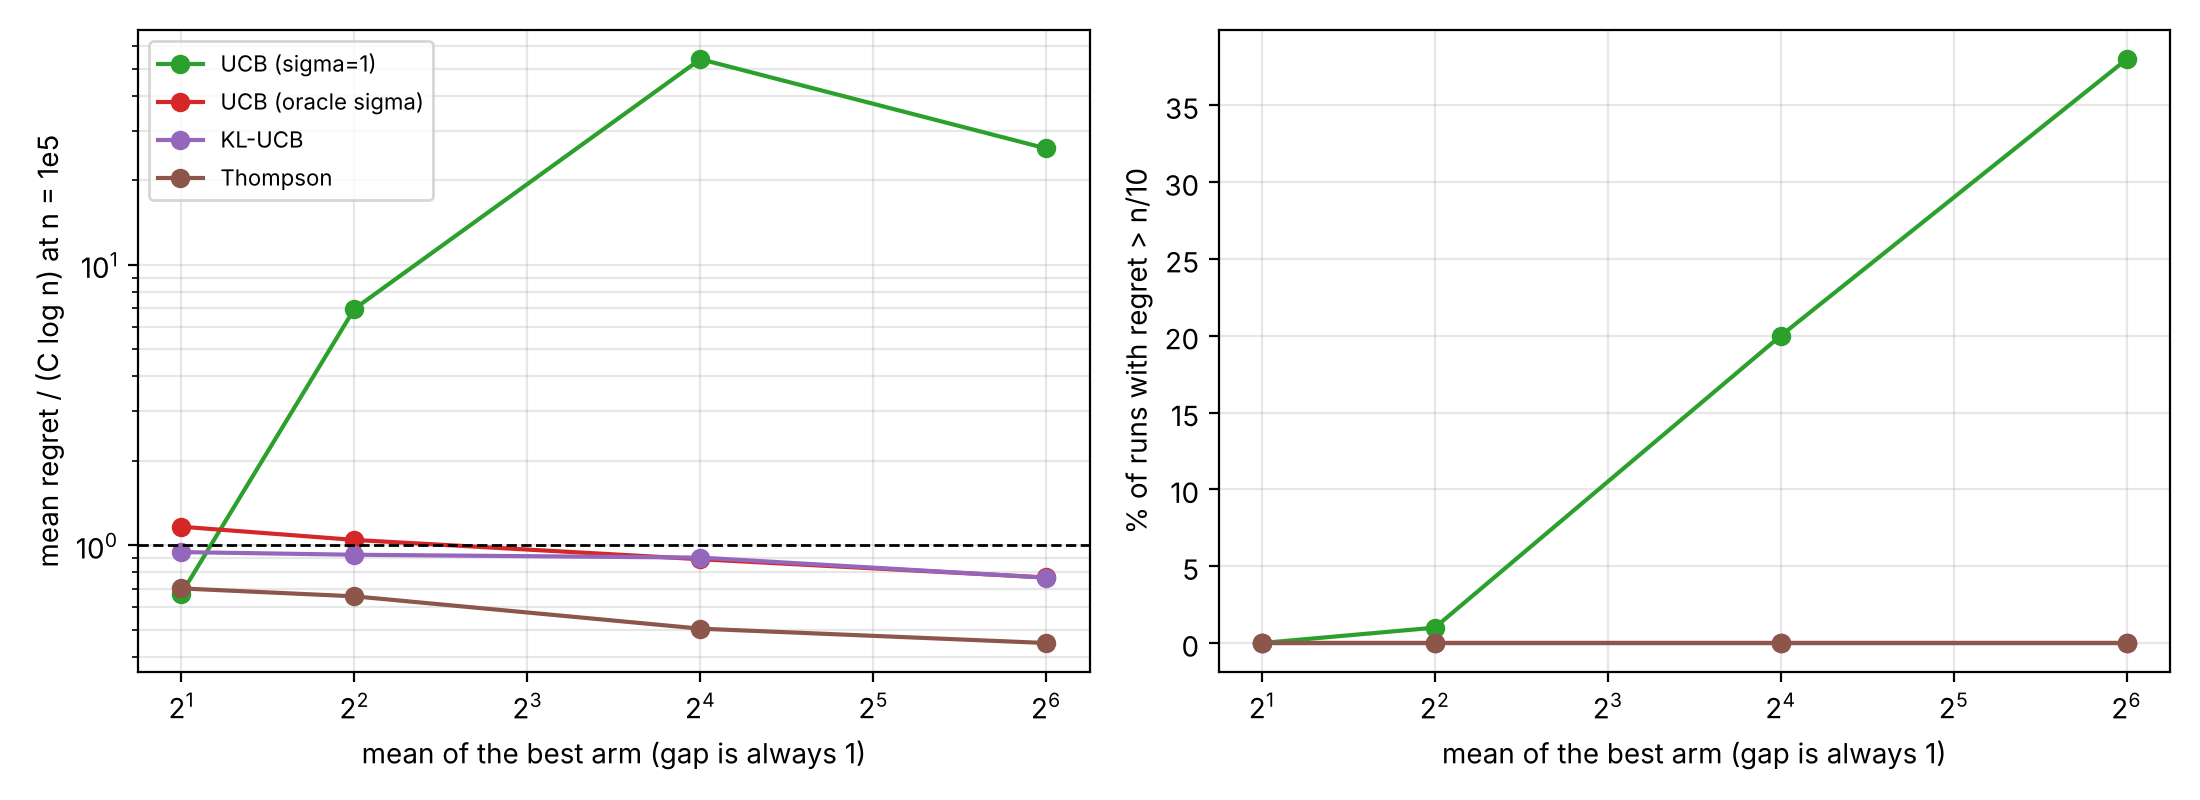
\includegraphics[width=\textwidth]{bandits_scale.png}
\caption{Left: mean regret divided by $C\log n$ at $n = 10^5$. Right: share of runs with regret above $n/10$.}
\label{fig:scale}
\end{figure}

Table~\ref{tab:scale} is quite brutal for UCB with $\sigma = 1$. Its median regret stays around 20 on every instance, which is far under $C \log n$ (about 18 times under it for $\mu = 16$ and 60 times for $\mu = 64$). If you only looked at medians, or at a few runs, you would think it is the best algorithm by far. But the share of runs stuck on the bad arm goes $0\%$, $1\%$, $20\%$, $38\%$, and the mean regret is 54 and 26 times the bound for the two largest instances. The confidence bonus $\sqrt{2\log t/N}$ is simply too small when the real standard deviation is 4 or 8: after a few unlucky pulls of the best arm, its index can stay under the other one for a very long time. This is exactly the price the Lai--Robbins bound talks about. The algorithm is very good on some instances because it is not uniformly good.

The oracle UCB behaves as the Gaussian approximation predicts. On $\mu = 2$ it is clearly worse than KL-UCB (43.7 against 35.5), because there the Poisson law is far from Gaussian and $2\mu = 4$ is larger than $C = 3.26$. From $\mu = 16$ on it is as good as KL-UCB. Of course it needs to know the variance, while KL-UCB gets it for free from the shape of the KL.

Among the algorithms that never get stuck, Thompson sampling is the best everywhere and by a lot: at $n = 10^5$ its mean regret is between $0.45$ and $0.70$ times $C\log n$. Like for the long run on $(2, 3, 4)$, this is not a contradiction but a sign that we are still far from the asymptotic regime. The local slopes between $10^3$ and $10^5$ say the same thing. For KL-UCB they are all above $C$ (1.3 to 1.6 times $C$), for Thompson sampling all below (0.6 to 0.85 times $C$). Both algorithms are supposed to end at the same constant, but they come from opposite sides, and on these problems the side of Thompson sampling is the comfortable one.

